\documentclass{article}
\usepackage{algorithmicx}
\usepackage{algpseudocode}
\usepackage{graphicx}

\begin{document}
{\noindent \Huge Problema a resolver:}
\newline \newline  El problema esta dado por la siguiente situaci\'on: nos encontramos en un extremo de un puente (afuera de \'el) y queremos llegar al otro extremo, bajo ciertas circunstancias y, si es posible hacer esto, hacerlo de la "mejor manera" (mas adelante se detallar\'a qu\'e significa esto y por qu\'e podr\'ia no ser posible atravesar el puente). El puente est\'a hecho con una cantidad \textit{n} de tablones seguidos y, algunos de ellos pueden estar rotos. Cuando esto suceda, vamos a querer saltar estos tablones rotos al atravesar el puente, pisando siempre tablones sanos cuando estemos avanzando.\newline
Tenemos una cantidad fija tablones seguidos que podemos saltar, la denominaremos \textit{c}, as\'i podemos ver que, si el puente tiene, en alg\'un momento, una cantidad \textit{$k > c$} de tablones rotos \textbf{seguidos}, entonces claramente no tendremos manera de atravesarlo ya que, intuitivamente, podemos pensar que, en el mejor de los casos (donde mejor significa estar lo m\'as alejados posibles del comienzo del puente) podr\'iamos estar en el tablon sano anterior (anterior inmediato) al primero de esos \textit{k} tablones rotos y, a\'un as\'i no podr\'iamos atravesar el puente ya que no podemos saltar m\'as de \textit{c} tablones seguidos, por lo tanto en cualquier otro caso (donde nos encontr\'aramos en un tabl\'on anterior al anterior inmediato del primero de los \textit{k} rotos por ejemplo), estar\'iamos en una situaci\'on similar porque eventualmente llegar\'iamos al tabl\'on sano que es el anterior inmediato al primero de los \textit{k} y quedar\'iamos estancados de la misma manera.
\newline En el caso en el que no se de la situaci\'on descripta anteriormente (es decir, en el caso en el cual s\'i podamos atravesar el puente), vamos a querer dar la menor cantidad de saltos (la "mejor manera").
\newline \newline Presentamos algunos ejemplos graficos junto a sus soluciones y las secuencias que lo representan. Los circulos con el A y el B determinan el punto de partida y el punto de llegada, ambos fuera del puente. Los tablones rotos est\'an pintados de negro.

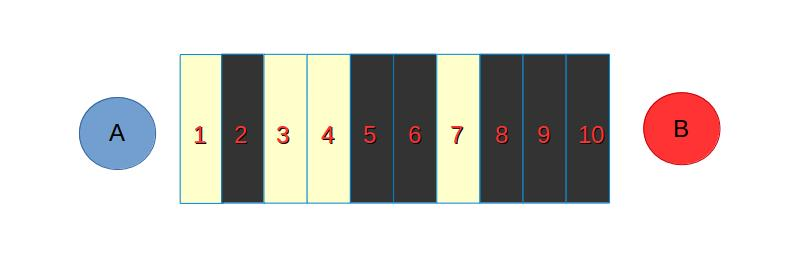
\includegraphics[width=\textwidth,height=\textheight,keepaspectratio
]{ejemplopuente1.jpg}
\begin {flushleft}
En este ejemplo, \textit{$n = 10$} y el puente se escribe como 10 c 0 1 0 0 1 1 0 1 1 1.
\newline Si \textit{$c = 3$}, entonces la soluci\'on est\'a dada por caer en los tablones 4 7 11. Notar que en realidad no existe un trabl\'on numerado con el 11, pero cuando exista una soluci\'on, para indicar que llegamos al punto de llegada, diremos que saltamos a un tabl\'on mayor estricto que la cantidad de tablones del puente (o sea, que estamos efectivamente fuera del puente).
Si tuvieramos el mismo puente pero con \textit{$n = 2$}, claramente no existir\'ia una soluci\'on ya que, si bien podr\'iamos llegar al tabl\'on 7 sin problemas, una vez ah\'i no tendr\'iamos manera de saltar el 8, 9 y 10 que est\'an rotos.\end {flushleft}
\vspace{1cm}
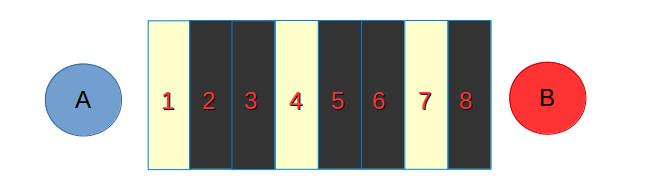
\includegraphics[width=\textwidth,height=\textheight,keepaspectratio
]{ejemplopuente2.jpg}
\begin {flushleft}Este otro puente se representa como 8 c 0 1 1 0 1 1 0 1.
\newline Si \textit{$c = 2$} entonces la soluci\'on es 1 4 7 9.
\newline Si \textit{$c = 1$} entonces no habr\'ia soluci\'on ya que hay 2 tablones rotos seguidos (esto ocurre dos veces en este caso particular pero con que ocurra una ya no hay soluci\'on posible).
\newline Si \textit{$c = 3$} la soluci\'on es  4 7 9.
\end {flushleft}

\vspace{1cm}
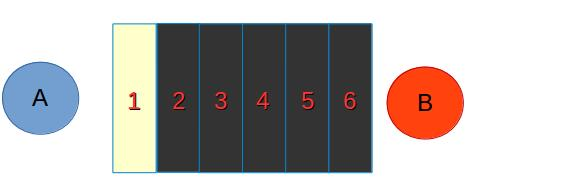
\includegraphics[width=\textwidth,height=\textheight,keepaspectratio
]{ejemplopuentes3.jpg}
\begin {flushleft}
Finalmente introducimos este ultimo ejemplo del puente 6 c 0 1 1 1 1 1.
Siguiendo la misma l\'ogica que ven\'iamos teniendo, podemos ver que este puente no tiene soluci\'on para \textit{$c < 5$}. Si \textit{$c = 5$} entonces la soluci\'on es 1 7 y s\'i \textit{$c > 5$} la soluci\'on es 7.
\end{flushleft}
\newpage
{\noindent \Huge Resoluci\'on:}
\newline \newline
La idea basicamente es ir recorriendo el puente (tabl\'on por tabl\'on) e ir almacenanando cual es el \'ultimo tabl\'on sano (lo llamaremos \textit{ultimosano}) desde el comienzo del puente hasta el tabl\'on de la iteraci\'on actual \textit{i} (notar que \textit{ultimosano} podr\'ia ser \textit{i}), los tablones que conformar\'ian la soluci\'on en el caso de que exista y la cantidad de tablones por los que pasamos desde el \'ultimo tabl\'on que agregu\'e a la soluci\'on (sin contarlo) hasta el tabl\'on de la iteraci\'on actual (cont\'andolo), llamaremos a esta \'ultima variable \textit{saltados}.
\newline Eventualmente podemos llegar a una iteraci\'on donde \textit{$saltados = c + 1$} (\textit{c} es dato y representa la cantidad de tablones como m\'aximo que puedo saltar) y, si no llegamos a esta iteraci\'on quiere decir que terminamos de recorrer todos los tablones del puente antes de llegar a pasar por \textit{$c + 1$} tablones desde el \'ultimo sano.
\newline Analicemos el primer caso donde efectivamente llegamos a esa iteraci\'on donde vale \textit{$saltados = c + 1$}: si llegamos a este punto significa que estamos parados en el tabl\'on mas lejano al cual puedo llegar saltando desde el \'ultimo tabl\'on que agregu\'e a la soluci\'on (porque si puedo saltar \textit{c} tablones seguidos desde donde estoy, entonces caigo en el tabl\'on \textit{$c + 1$}). Entonces nuevamente pueden pasar dos cosas: 1) \textit{$i - ultimosano > c$} (que la cantidad de tablones entre el tabl\'on de la iteraci\'on actual \textit{i} hasta \textit{ultimosano} sea mas grande que c) 2) \textit{$i - ultimosano <= c$}. Si estamos en 1) voy a tener una cantidad mayor estricta que \textit{c} de tablones seguidos donde ninguno de ellos es un tabl\'on sano (la \'ultima vez que asign\'e un valor a \textit{ultimosano} fue o bien antes de empezar a iterar, o sea cuando estoy fuera del puente, o en un tabl\'on que dista a m\'as de \textit{c} tablones del actual), esto quiere decir que est\'an todos rotos y, como no puedo saltar una cantidad mayor que \textit{c} de tablones seguidos, concluimos que no existe una soluci\'on al problema. Ahora bien si estamos en 2), entonces quiere decir que existe un tabl\'on sano (y est\'a almacenado en \textit{ultimosano} entre el \'ultimo que agregu\'e a la soluci\'on  (si no agregu\'e ninguno, entonces este tabl\'on representa el punto de partida fuera del puente) y el tabl\'on representado por la iteraci\'on actual \textit{i} y este tabl\'on NO es el \'ultimo que agregu\'e a la soluci\'on (de ser as\'i no estar\'iamos en este caso). Entonces lo que hacemos es agregar \textit{ultimosano} a la soluci\'on y actualizar el valor de \textit{saltados} para que represente la cantidad de tablones que salt\'e desde el \'ultimo que agregu\'e a la soluci\'on (que es el que agregamos reci\'en, \textit{ultimosano}) hasta llegar al tabl\'on de la iteraci\'on actual \textit{i}. Una vez hecho esto, repetimos el proceso descripto con la siguiente iteraci\'on.
\newline
Dado que los tablones que deben ser soluci\'on se agregan a la misma cuando nos encontramos en una iteraci\'on \textit{i} en la cual vale \textit{$saltados = c + 1$}, podr\'ia suceder que terminemos de iterar y no hayamos pasado por esta iteraci\'on \textit{i}. Esto quiere decir que a partir del \'ultimo tabl\'on que agregu\'e a la soluci\'on, hay una cantidad menor estricta que \textit{$c + 1$} tablones y por lo tanto, puedo saltarlos todos, alcanzando as\'i el punto de llegada fuera del puente.
\newline Cuando terminamos de iterar todos los tablones del puente, agregamos como el \'ultimo "tabl\'on" de la soluci\'on, un n\'umero mayor estricto que \textit{n} para indicar que estamos fuera del puente. 

A continuaci\'on, presentamos el pseudoc\'odigo que hace lo que describimos arriba:
\vspace{0.4cm}
\begin{algorithmic}[1]
\Procedure{ResolverPuente}{$puente,c$}
	\State $ultimosano\gets -1$
	\State $saltados\gets 0$
	\State $output\gets \emptyset$
	\State $n\gets cantidadTablones(puente)$
	\For{$i\gets 0, n - 1$}
		\State $saltados++$
		\If{$puente[i]\gets 0$}
			\State $ultimosano\gets i$
		\EndIf
		\If{$saltados = c + 1$}
			\If{$i - ultimosano > c \vee ultimosano == - 1$}
				\State no hay soluci\'on, termino
			\EndIf
			\State $agregar(output, i + 1)$
			\State $saltados = i - ultimosalto$
		\EndIf
	\EndFor
	\State $agregar(output$, size($puente$) + 1)
\EndProcedure
\end{algorithmic}
\vspace{1cm}
{\noindent \Huge Demostraci\'on de correctitud:}
\newline
\newline Para realizar la demostraci\'on de correctitud del algoritmo, vamos a separarla en dos casos: cuando el problema no tiene soluci\'on (caso I) y cuando s\'i tiene (caso II).
\newline
\newline Caso I) Queremos probar que: 1)si el algoritmo informa que el problema no tiene soluci\'on, entonces efectivamente el problema no tiene soluci\'on y 2)no puede pasar que el problema no tenga soluci\'on y el algoritmo no lo informe, devolviendo as\'i, una soluci\'on incorrecta.
\newline  1) Dado que nuestro algoritmo informa que el problema no tiene soluci\'on cuando vale A: $(saltados = c + 1) \wedge (i - ultimosano > c \ \vee \ ultimosano == -1)$ y $A\Rightarrow (i - ultimosano > c \ \vee \ ultimosano == -1) = B$, como en cada iteraci\'on sabemos el \'indice del \'ultimo tabl\'on sano porque vamos pisando la variable $ultimosano$ (l\'ineas 8 a 10 del pseudoc\'odigo), $B$ nos est\'a diciendo que entre el tabl\'on de la iteraci\'on actual y el \'ultimo tabl\'on sano que mir\'e, hay una cantidad \textbf{estrictamente mayor a $c$} de tablones, por lo tanto nunca voy a poder saltarlos, ya que si estoy parado en el tabl\'on $ultimosano$, vemos que hay mas de $c$ tablones para saltar y no puedo y, la otra opci\'on es que est\'e parado en un tabl\'on anterior a $ultimosano$, y eventualmente llegar\'ia, como muy lejos, al tabl\'on $ultimosano$ sin caerme. Nunca voy a poder estar en un tabl\'on posterior a $ultimosano$, por lo tanto concluimos que el problema no tiene soluci\'on.
\newline 2)Para que el algoritmo no tenga soluci\'on, tiene que pasar que haya una cantidad $k > c$ de tablones rotos seguidos ya que si esto no pasa, entonces siempre puedo avanzar y caer en un tabl\'on sano m\'as adelante del que estoy parado y, eventualmente voy a poder saltar al punto de llegada fuera del puente.
Llamemos $j$ al primer tabl\'on de esos $k$ tablones rotos seguidos. $j-1$ entonces representa el \'ultimo tabl\'on sano antes del primero de esos $k$ tablones rotos seguidos, o tambi\'en puede valer -1 en el caso de que esos $k$ tablones seguidos sean los primeros $k$ tablones del puente.
\newline Debido a que estamos recorriendo tabl\'on por tabl\'on, sabemos que en alg\'un momento vamos a caer en el tabl\'on $j + c$ (si no llegamos a este tabl\'on es porque nos dimos cuenta antes que no hab\'ia soluci\'on porque, antes de este tabl\'on sano $j - 1$, exist\'ian $k' > c$ tablones rotos seguidos) el cual existe ya que a partir de $j$ hay $k > c$ tablones seguidos y, en esa iteraci\'on va a valer A ya que se habr\'a incrementado $saltados$ en uno desde $j$ hasta la iteraci\'on actual $i$, y dado que $i = j + c$ y $ultimosano = j - 1 $, $ \Rightarrow i - ultimosano \equiv  j + c - (j - 1) =  c + 1 > c$ y como vale $A$ entramos en el if de la l\'inea 12, indicando as\'i que no hay soluci\'on.

\vspace{1cm} \noindent Caso II) Como ya demostramos que el algoritmo funciona correctamente cuando el problema no tiene soluci\'on y ahora queremos ver que tambi\'en funcione correctamente cuando s\'i la tiene, vamos a asumir de ahora en m\'as que $existe$ una soluci\'on al problema.
\newline Vimos que una soluci\'on al problema no es m\'as que un conjunto (de cardinal m\'inimo) de tablones sanos del puente, en el cual si sacamos un tabl\'on y el tabl\'on pr\'oximo a \'el (el que le sigue en \'indice), la cantidad de tablones entre ellos es menor o igual a $c$ y, adem\'as, este conjunto contiene al punto de llegada fuera del puente, indentificado como un tabl\'on m\'as de \'indice mayor a la cantidad de tablones del puente. Entonces, ser\'ia similar si pens\'aramos a la soluci\'on como ese mismo conjunto descripto anteriormente, menos el tabl\'on que representa el punto de llegada y, que ademas cumple que la cantidad de tablones desde el tabl\'on con mayor \'indice (sin contarlo) hasta el \'ultimo tabl\'on del puente (cont\'andolo), es menor o igual a c. Y ese ser\'a nuestro concepto de soluci\'on para hacer la siguiente demostraci\'on (pasar de ese conjunto a la salida que pide el problema que tenga el algoritmo es trivial, ya que basta solo con agregarle un \'indice mayor a $n$ al conjunto).
\newline Vamos a querer probar que, al finalizar el for, $output$ va a ser un conjunto que cumpla con lo que dijimos reci\'en (*).

\vspace{0.5cm}\noindent Decimos que un conjunto $S$ es subsoluci\'on de una soluci\'on $S'$, cuando $S \subseteq S'$.
\newline Para poder probar (*), vamos a demostrar que I)$output$ comienza siendo subsoluci\'on de una soluci\'on $S$ y II)al comenzar y finalizar cada iteraci\'on, $output$ sigue siendo subsoluci\'on de alguna soluci\'on (no necesariamente siempre la misma)

\vspace{0.3cm}\noindent I)Vale trivialmente, ya que asumimos que el problema tiene soluci\'on y, como $output$ comienza siendo el cojunto vac\'io y sabemos que vale $(\emptyset \subseteq C)(\forall \ C)$, entonces particularmente vale para $C = S$

\vspace{0.4cm}\noindent II)Si al finalizar la iteraci\'on $i$, $output$ no cambi\'o con respecto a su valor antes de empezar dicha iteraci\'on, entonces claramente sigue valiendo que $output$ es subsoluci\'on de una soluci\'on S, ya que $output$ empieza si\'endolo. \newline Ahora bien, si $output$ s\'i cambi\'o de valor, significa que se agreg\'o el tabl\'on $ultimosano$ (no puede cambiar de otra manera) y pueden ocurrir dos cosas: que $ultimosano \in S$ (siendo $S$ la soluci\'on que ten\'ia a $output$ como subsoluci\'on antes de que cambie su valor) y en tal caso $output$ seguir\'ia siendo subsoluci\'on de $S$ porque antes lo era y ahora agregamos un elemento que pertenece a $S$, o que $ultimosano \notin S$. Analicemos este \'ultimo caso: llamemos $t$ al \'ultimo tabl\'on que agregu\'e a $output$ (antes de que cambie su valor en esta iteraci\'on) y $r$ al tabl\'on pr\'oximo a $t$ de $S$. Dado que $r \neq ultimosano$, entonces necesariamente $r < ultimosano$, ya que $ultimosano$ es el tabl\'on sano m\'as lejano a $t$, entonces podemos tomar $S' = (S \ \backslash \ r) \ \cup \ \{ultimosano\}$ y $S'$ efectivamente es una soluci\'on ya que desde $t$ puedo saltar a $ultimosano$ ($ultimosano$ se encuentra, a lo sumo a $c$ tablones mas adelante de $t$) y, desde $ultimosano$ puedo saltar a los mismos tablones que podr\'ia saltar desde $r$ y m\'as tambi\'en. Concluimos entonces que, como $output \subseteq S'$ y $S'$ es soluci\'on, $output$ sigue siendo subsoluci\'on de una soluci\'on.

\vspace{0.4cm}\noindent Cuando finalice la \'ultima iteraci\'on del ciclo, el \'ultimo tabl\'on que habr\'e agregado (llam\'emoslo $m$) estar\'a a lo sumo a $c$ tablones del final del puente ya que si no, hubieramos llegado al tabl\'on $m + c + 1$ e informar\'iamos que no hay soluci\'on ya que la distancia a $ultimosano$ es mayor que $c$ y esto no puede pasar ya que asumimos que exixte una soluci\'on), y probamos que $output$ es subsoluci\'on de una soluci\'on al iniciar y finalizar cada iteraci\'on, por lo tanto tambi\'en lo es al terminar el ciclo. Como no necesitamos agregar otro tabl\'on m\'as porque ya podemos saltar desde el \'ultimo tabl\'on agregado al punto de llegada, entonces efectivamente $ultimosano$ es una soluci\'on.

\vspace{1.5cm}
{\noindent \Huge Complejidad temporal:}
\newline \newline
La complejidad del algoritmo es claramente lineal a la cantidad de tablones, ya que todas las operaciones que se hacen dentro del ciclo son de orden constante (en el c\'odigo fuente almacenamos la soluci\'on en el tipo std::list, el cual tiene orden constante en la inserci\'on seg\'un http://en.cppreference.com/w/cpp/container/list y para almacenar el puente utilizamos std::vector<int> el cual tiene orden constante en el acceso a una posici\'on seg\'un http://en.cppreference.com/w/cpp/container/vector). Todas las dem\'as operaciones realizadas son if's y asignaciones/sumas de enteros, que tambi\'en tienen \'ordenes de complejidad constantes.
\newline El peor caso del algoritmo entonces, es cuando tiene soluci\'on, ya que si pasa eso entonces debe recorrer necesariamente todos los tablones (no sale antes del ciclo) y es $\theta (n)$.
\newline El mejor caso del algoritmo, es cuando no tiene soluci\'on y los primeros $k > c$ tablones seguidos, son los primeros $k$ tablones del puente, en tal caso el algoritmo tendr\'ia un tiempo de $\theta (k)$ donde $c < k \le n$.

\vspace{1.5cm}
{\noindent \Huge Mediciones de tiempo:}
\newline \newline Para medir la performance del algoritmo se han generado dos conjuntos de 30 instancias cada uno. La instancia $i$ de cada conjunto tiene $n = i * 1.000.000$ (o sea van de un mill\'on a treinta millones de tablones) y el salto m\'aximo $c$, tambi\'en elegido de manera aleatoria, est\'a en el rango [0, 999.999].
\newline La diferencia entre los dos conjuntos radica en que, en un conjunto (R), la probabilidad de que un tabl\'on est\'e roto es 0.99 y en otro (S) es 0.5. De esta manera, intuitivamente podemos ver que en el conjunto S, es muy poco probable que una instancia del problema no tenga soluci\'on.
\newline Cada una de las instancias de cada conjunto fue resuelta (o no) por el algoritmo 10 veces y se registraron los tiempos de cada ejecuci\'on, tomando el m\'inimo, m\'aximo y promedio de tiempo de cada una de las 10 ejecuciones de cada instancia.
\newline\newline Presentamos los gr\'aficos de tiempo para el conjunto S:

\vspace{0.5cm}
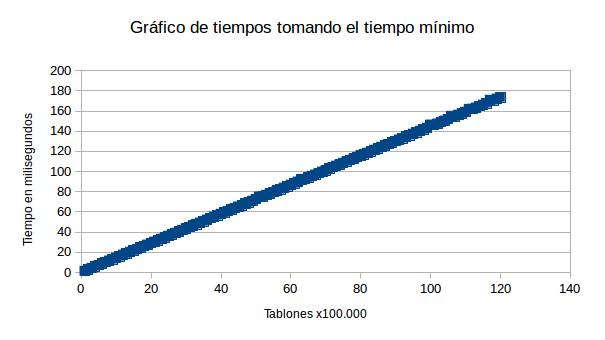
\includegraphics[width=\textwidth,height=\textheight,keepaspectratio
]{puentetiempominimoS.jpg}
\vspace{0.5cm}
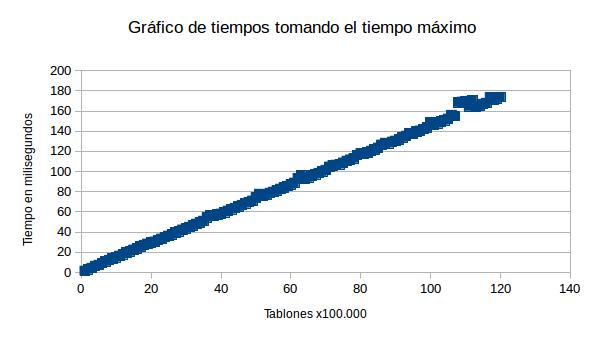
\includegraphics[width=\textwidth,height=\textheight,keepaspectratio
]{puentetiempomaximoS.jpg}
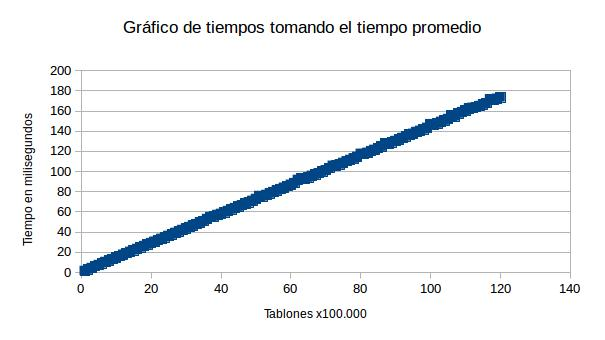
\includegraphics[width=\textwidth,height=\textheight,keepaspectratio
]{puentetiempopromedioS.jpg}

\end{document}